\section{Model Hammersteina}
Po przeanalizowaniu charakterystyki statycznej oraz porównaniu modelu nieliniowego z liniowym przystąpiono do identyfikacji modelu Hammersteina.
Istota polega na umieszczeniu nieliniowego bloku statycznego przed liniowym blokiem dynamicznym, co pozwala na oddzielenie nieliniowości od dynamiki systemu. Jego główną zaletą jest prostsza identyfikacja parametrów, ponieważ najpierw określa się charakterystykę statyczną, a dopiero potem analizuje dynamikę. Takie podejście lepiej odwzorowuje systemy, w których nieliniowości wynikają z właściwości aktuatorów lub czujników, a część dynamiczna pozostaje liniowa. Graficzne ujęcie opisanego modelu zilustrowano na rys. \ref{hamm_model}.

\begin{figure}[h!]
\centering
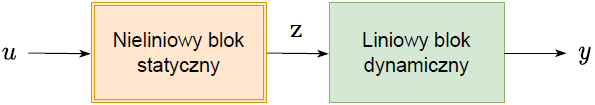
\includegraphics[width=\textwidth]{pictures/hamm_model}
\caption{Reprezentacja graficzna modelu Hammersteina.}
\label{hamm_model}
\end{figure}

\noindent Cała procedura w przypadku analizowanego obiektu wygląda następująco, sygnał sterujący jest wejściem nieliniowego bloku statycznego, którego wyjściem jest przekonwertowany sygnał $z = f(u)$. Następnie sygnał $z$ trafia do liniowego bloku dynamicznego. Dzięki temu rozdzieleniu nieliniowości i dynamiki, możliwe jest zastosowanie klasycznych metod projektowania regulatorów dla części dynamicznej, co upraszcza proces sterowania.

\subsection{Nieliniowy blok statyczny}
Nieliniowość w charakterystyce statycznej została wprowadzono za pomocą logiki rozmytej (ang. \textit{fuzzy logic}), a konkretnie za pomocą modeli rozmytych Takagi-Sugeno. Zastosowano dwa podejścia, jedno standardowe z następnikami liniowymi, natomiast drugie z następnikami hiperbolicznymi.

\subsection{Następniki liniowe}
W standardowej wersji modeli Takagi-Sugeno następniki przyjmują liniową postać, dlatego to właśnie od nich postanowiono zacząć. Rozmyto zmienną wejściową oraz wybrano odpowiednią liczbę zbiorów rozmytych. Zastosowano następniki liniowe postaci:

\begin{equation}
\begin{aligned}
\text{Reguła 1: Jeśli} \quad u(k) \quad \text{jest} \quad &U_1, \quad \text{to}: \quad y^1(k) = a_1 u(k) + b_1 \\[10pt]
\text{Reguła 2: Jeśli} \quad u(k) \quad \text{jest} \quad &U_2, \quad \text{to}: \quad y^2(k) = a_2 u(k) + b_2 \\[10pt]
&\vdots \\[10pt]
\text{Reguła 5: Jeśli} \quad u(k) \quad \text{jest} \quad &U_5, \quad \text{to}: \quad y^2(k) = a_5 u(k) + b_5 \\[10pt]
\end{aligned}
\label{nastepniki_lin}
\end{equation}

\noindent Natomiast wyjście systemu rozmytego obliczano zgodnie ze wzorem \ref{wniosek}.

\newpage

\begin{figure}[h!]
\centering
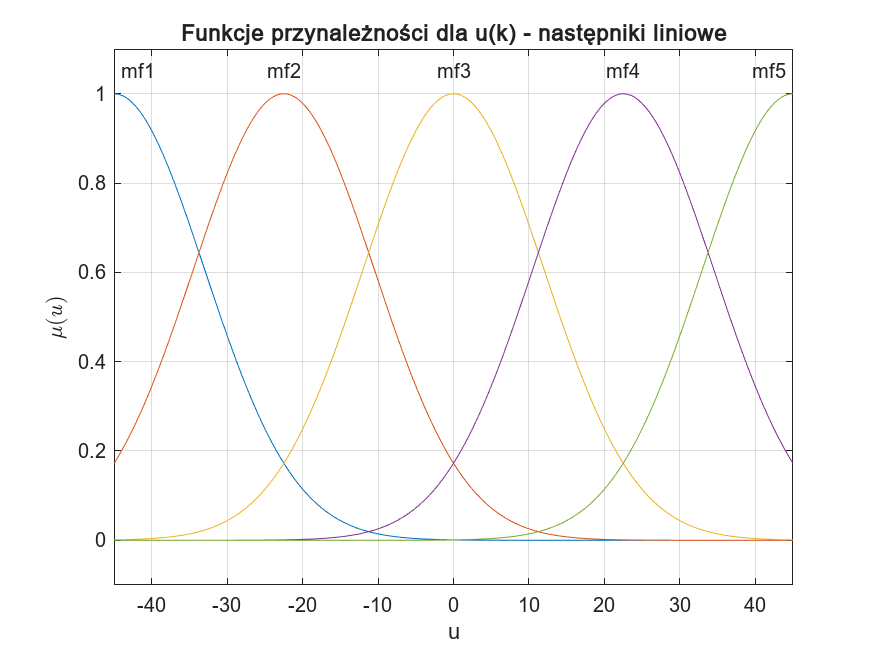
\includegraphics[width=\textwidth]{pictures/hamm_linearFis}
\caption{Zbiory rozmyte - następniki liniowe.}
\end{figure}

Zarówno do budowy modelu, jak i wyznaczenia parametrów następników wykorzystano narzędzia oferowane przez MATLAB w ramach \textit{Fuzzy Logic Toolbox}. Korzystając z funkcji \verb+sugfis()+ zbudowano nieliniowy model rozmyty typu Takagi - Sugeno. Zdecydowano się na pięć zbiorów rozmytych o gaussowskim kształcie, co zapewnia różniczkowalność (SZAU). Następnie, dzięki wykorzystaniu \verb+addInput()+, \verb+addOutput()+, \verb+addMF()+ udało się zbudować bazę reguł - \verb+addRule()+, co bezpośrednio przełożyło się na wyznaczenie współczynników pierwszej iteracji. Konieczne było późniejsze ręczne dostrajanie modelu, które przy względnie dużej liczbie zbiorów nie przysporzyło dużo problemów. Ostatecznie zdefiniowano następujące wartości parametrów następników:

\begin{table}[h!]
\centering
\renewcommand{\arraystretch}{1.2} % Zwiększa wysokość wierszy
\begin{tabular}{|>{\centering\arraybackslash}m{3cm}|>{\centering\arraybackslash}m{3cm}|>{\centering\arraybackslash}m{3cm}|}
\hline
Nr reguły & Współczynnik $a_r$ & Współczynnik $b_r$ \\ \hline
1 & $\num{0.7895}$ & $\num{0.0001}$ \\ \hline
2 & $\num{0.8982}$ & $\num{0.0002}$ \\ \hline
3 & $\num{1.0933}$ & $\num{0.0001}$ \\ \hline
4 & $\num{1.0489}$ & $\num{0}$ \\ \hline
5 & $\num{1.2034}$ & $\num{0.0001}$ \\ \hline
\end{tabular}
\end{table}

\newpage

\subsection{Następniki nieliniowe}
Wprowadzając następniki w postaci hiperbolicznej spodziewano się zachowania dokładności przy jednoczesnym zmniejszeniu liczby zbiorów rozmytych [Robust observer-based controller design for Takagi–Sugeno systems with nonlinear consequent parts]. Sformułowano następującą bazę reguł:

\begin{equation}
\begin{aligned}
\text{Reguła 1: Jeśli} \quad u(k) \quad \text{jest} \quad &U_1, \quad \text{to}: \quad y^1(k) = a_1 \sinh\left(\frac{u(k)}{b_1}\right) \\[10pt]
\text{Reguła 2: Jeśli} \quad u(k) \quad \text{jest} \quad &U_2, \quad \text{to}: \quad y^2(k) = a_2 \sinh\left(\frac{u(k)}{b_2}\right) \\[10pt]
\text{Reguła 3: Jeśli} \quad u(k) \quad \text{jest} \quad &U_3, \quad \text{to}: \quad y^2(k) = a_3 \sinh\left(\frac{u(k)}{b_3}\right)
\end{aligned}
\label{nastepniki_nlin}
\end{equation}

Zgodnie z oczekiwaniami udało się wprowadzić mniejszą liczbę zbiorów rozmytych.

\begin{figure}[h!]
\centering
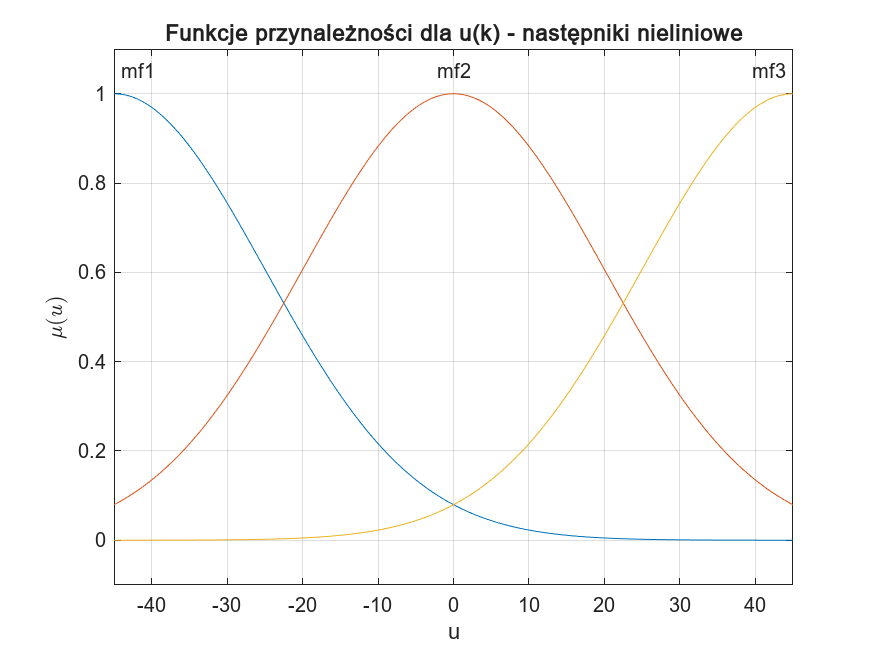
\includegraphics[width=\textwidth]{pictures/hamm_nonlinearFis}
\caption{Zbiory rozmyte - następniki nieliniowe.}
\end{figure}

\newpage

Procedura dostrajania parametrów następników różniła się w stosunku do odpowiedników liniowych. Wynikało to z tego, że wykorzystywane narzędzie do budowy modelu rozmytego domyślnie stroi parametry dla następników liniowych, stąd konieczność znacznej modyfikacji i ręcznego dostrajania. Następnie, po ręcznym dostrojeniu wykorzytsano funkcję z pakietu \textit{Optimization Toolbox}, mianowicie \verb+fminsearch()+. Wybrano taką kolejność ze względu na fakt, że odwracając kolejność, tzn. stosując najpierw metodę Neldera-Meada, otrzymywane wyniki były gorsze niż te wybrane ręcznie. Było to spowodowane skłonnością do wpadania algorytmu w minima lokalne. Istotnym aspektem w tym przypadku okazała się normalizacja argumentu, bowiem kształt funkcji $\sinh()$ zmienia się bardzo gwałtownie dla rosnących wartości zmiennej (rys. {\ref{sinh}}. 

\begin{figure}[h!]
\centering
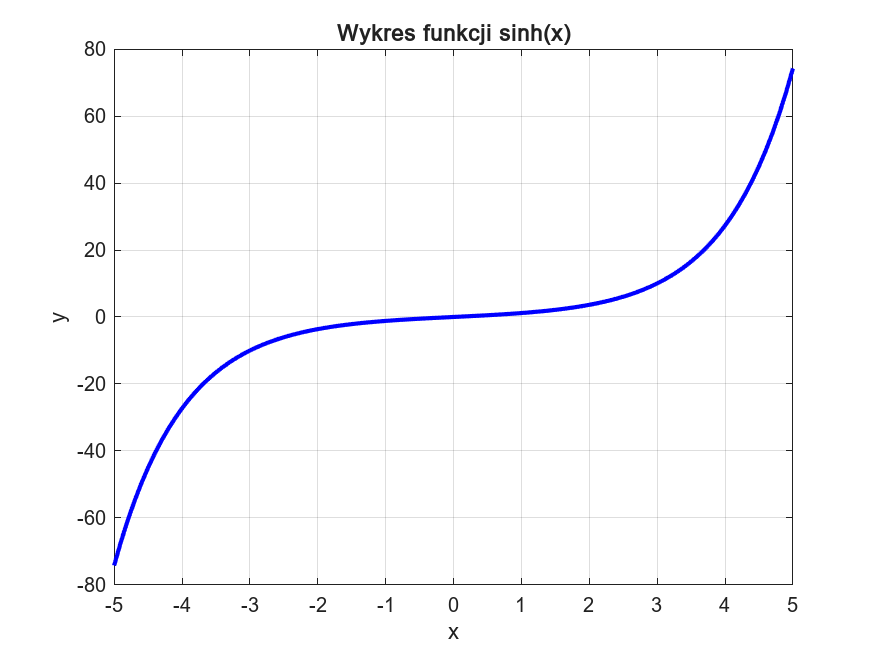
\includegraphics[width=\textwidth]{pictures/sinh}
\caption{Wykres funkcji $\sinh()$.}
\label{sinh}
\end{figure}

Ostateczne wartości współczynników następników reguł zebrano w tab. \ref{nonlinear_coeff}.

\begin{table}[h!]
\centering
\renewcommand{\arraystretch}{1.2} % Zwiększa wysokość wierszy
\begin{tabular}{|>{\centering\arraybackslash}m{2cm}|>{\centering\arraybackslash}m{3cm}|>{\centering\arraybackslash}m{3cm}|}
\hline
Nr reguły & Współczynnik $a_r$ & Współczynnik $b_r$ \\ \hline
1. & $\num{46.4941}$ & $\num{62.8862}$ \\ \hline
2. & $\num{36.2347}$ & $\num{36.2592}$ \\ \hline
3. & $\num{110.4841}$ & $\num{98.7690}$ \\ \hline    
\end{tabular}
\caption{Współczynniki hiperbolicznych następników reguł.}
\label{nonlinear_coeff}
\end{table}

\newpage

\subsection{Porównanie}
Dostroiwszy oba modele przyszedł czas na ich porównanie. Wygenerowano pięć sekwencji losowo zmieniającego się sygnału sterującego, następnie wynik został porównany do rezultatu uzyskanego dla modelu nieliniowego - wzorcowego - obliczonego za pomocą zmodyfikowanej metody Eulera. Wskaźnikiem porównawczym był błąd średnio kwadratowy. Aby zaznaczyć jakie korzyści wnosi nieliniowa część modelu Hammersteina na dokładność modelowania, w każdej sekwencji obliczono także wskaźnik dla modelu liniowego.

\begin{figure}[h!]
\centering
\subfloat[Następniki liniowe]{
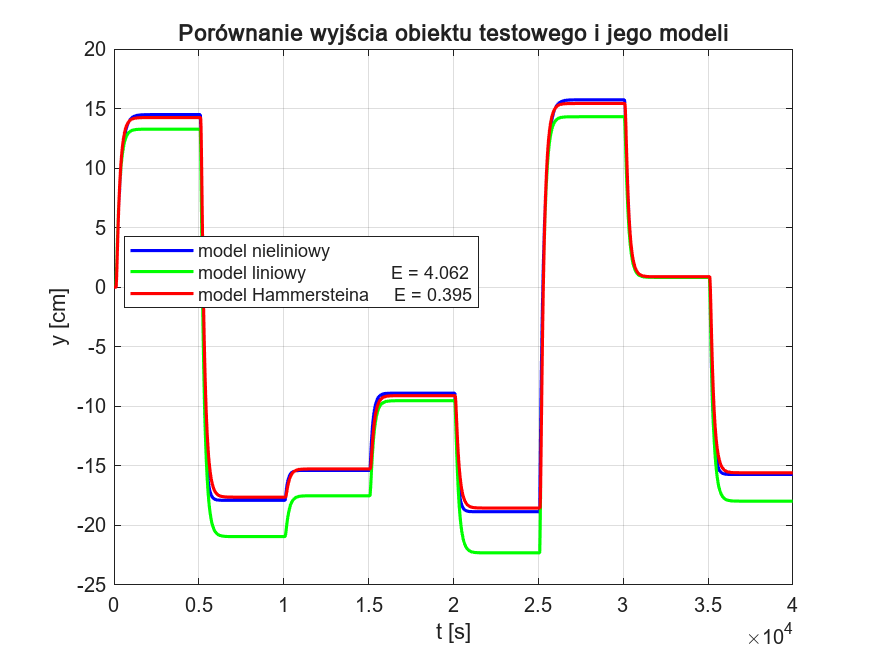
\includegraphics[width=0.7\textwidth]{pictures/HammersteinLinearModel_1}}
\vspace{0.5cm}
\subfloat[Następniki nieliniowe]{
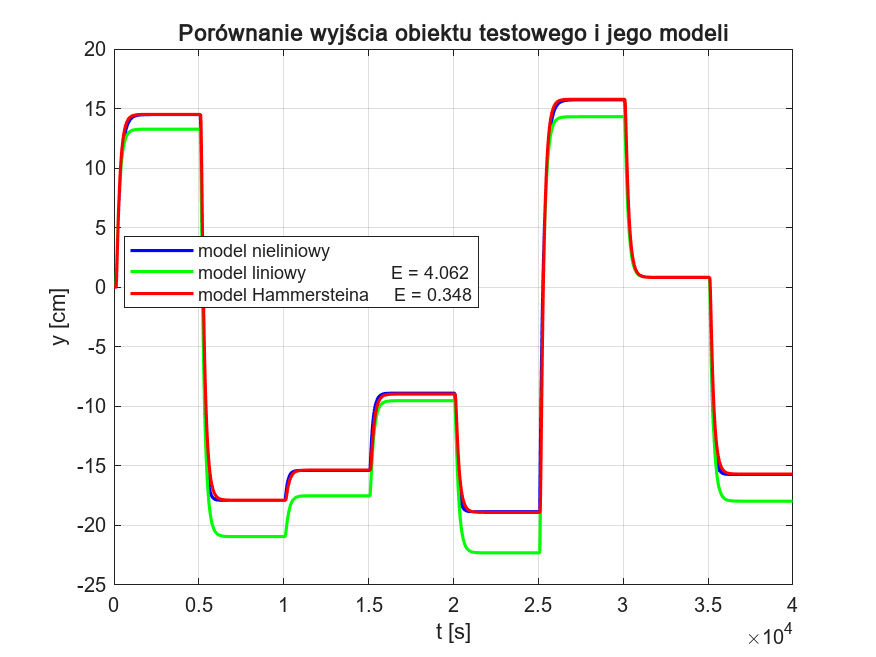
\includegraphics[width=0.7\textwidth]{pictures/HammersteinNonlinearModel_1}}
\caption{Porównanie modelu Hammersteina z następnikami liniowymi i nieliniowymi - pierwsza sekwencja.}
\label{first_hamm}
\end{figure}

\begin{figure}[p]
\centering
\subfloat[Następniki liniowe]{
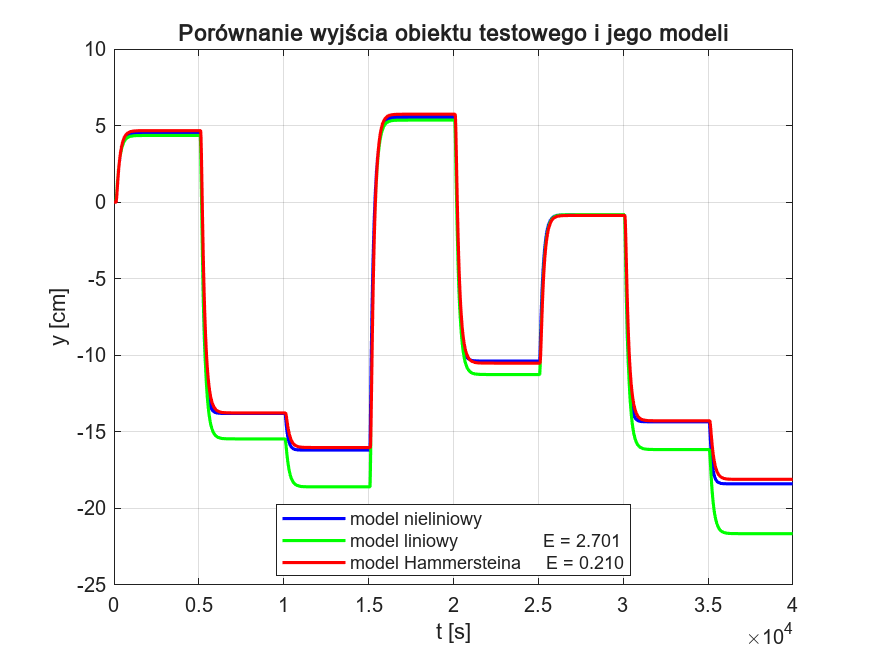
\includegraphics[width=0.75\textwidth]{pictures/HammersteinLinearModel_2}}
\vspace{0.5cm}
\subfloat[Następniki nieliniowe]{
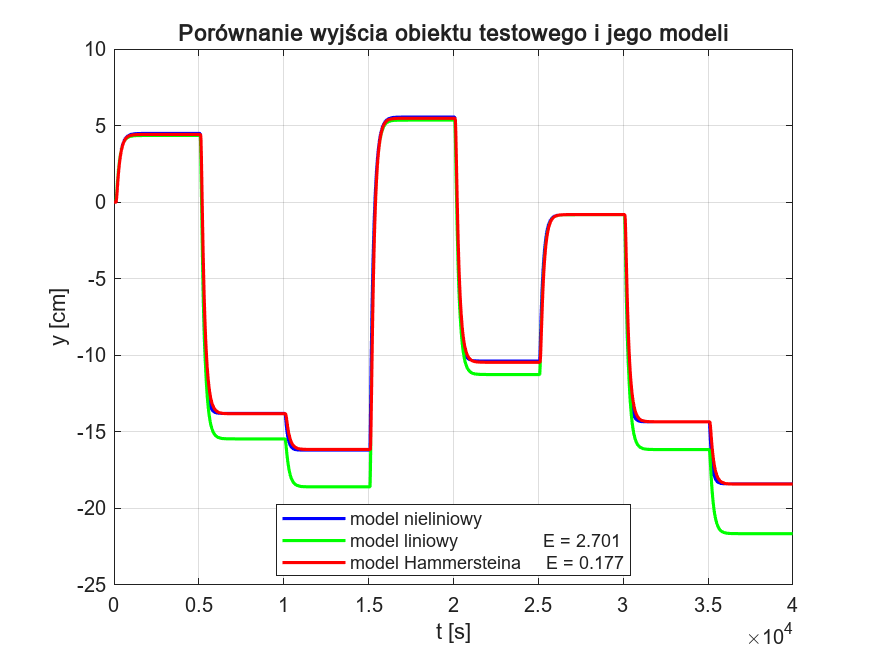
\includegraphics[width=0.75\textwidth]{pictures/HammersteinNonlinearModel_2}}
\caption{Porównanie modelu Hammersteina z następnikami liniowymi i nieliniowymi - druga sekwencja.}
\end{figure}

\begin{figure}[p]
\centering
\subfloat[Następniki liniowe]{
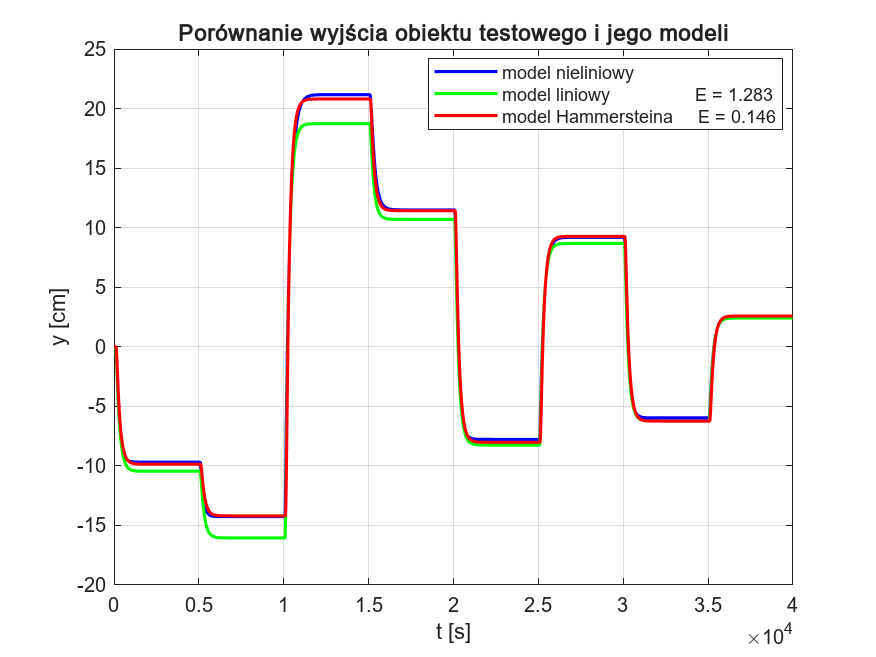
\includegraphics[width=0.75\textwidth]{pictures/HammersteinLinearModel_3}}
\vspace{0.5cm}
\subfloat[Następniki nieliniowe]{
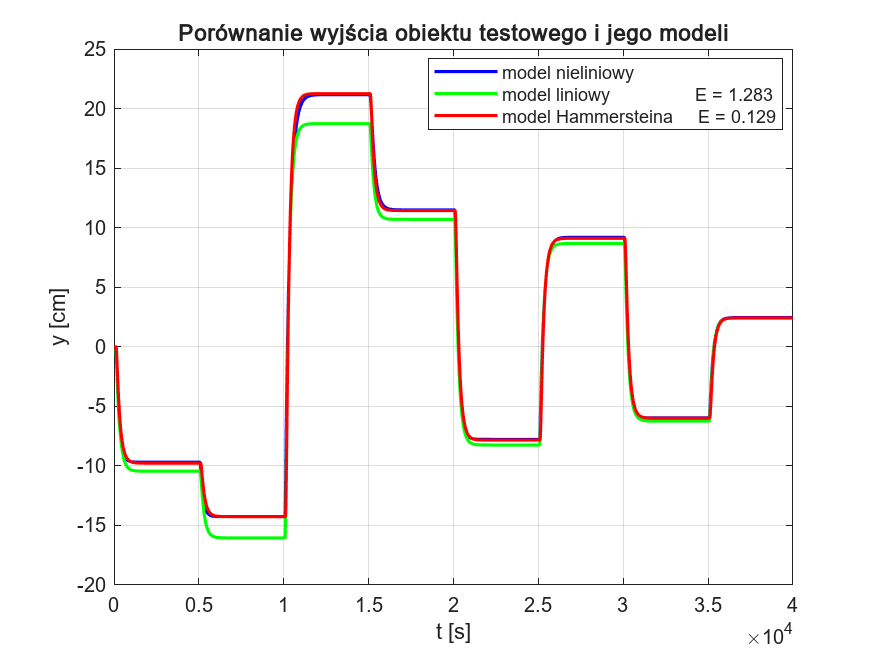
\includegraphics[width=0.75\textwidth]{pictures/HammersteinNonlinearModel_3}}
\caption{Porównanie modelu Hammersteina z następnikami liniowymi i nieliniowymi - trzecia sekwencja.}
\end{figure}

\begin{figure}[p]
\centering
\subfloat[Następniki liniowe]{
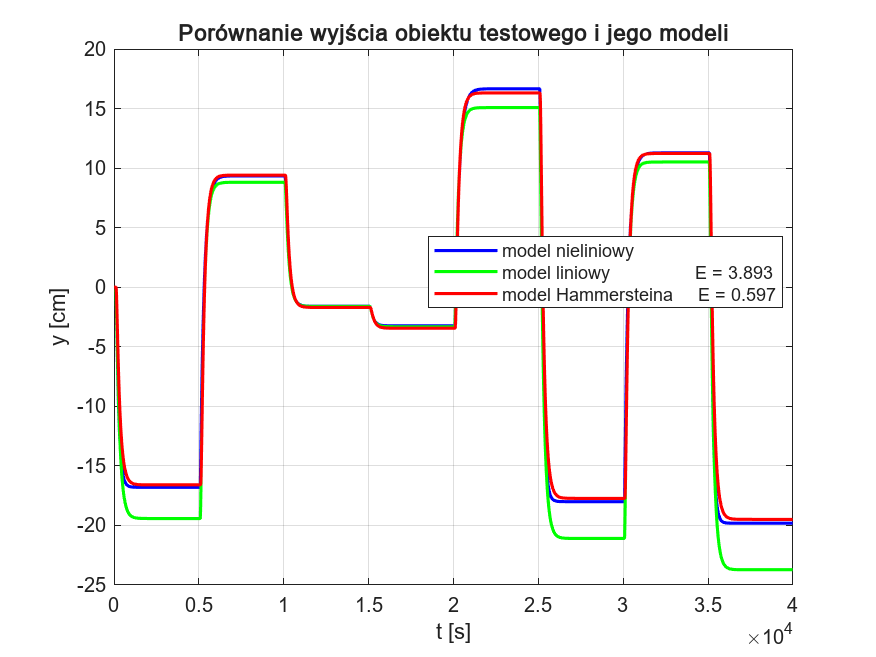
\includegraphics[width=0.75\textwidth]{pictures/HammersteinLinearModel_4}}
\vspace{0.5cm}
\subfloat[Następniki nieliniowe]{
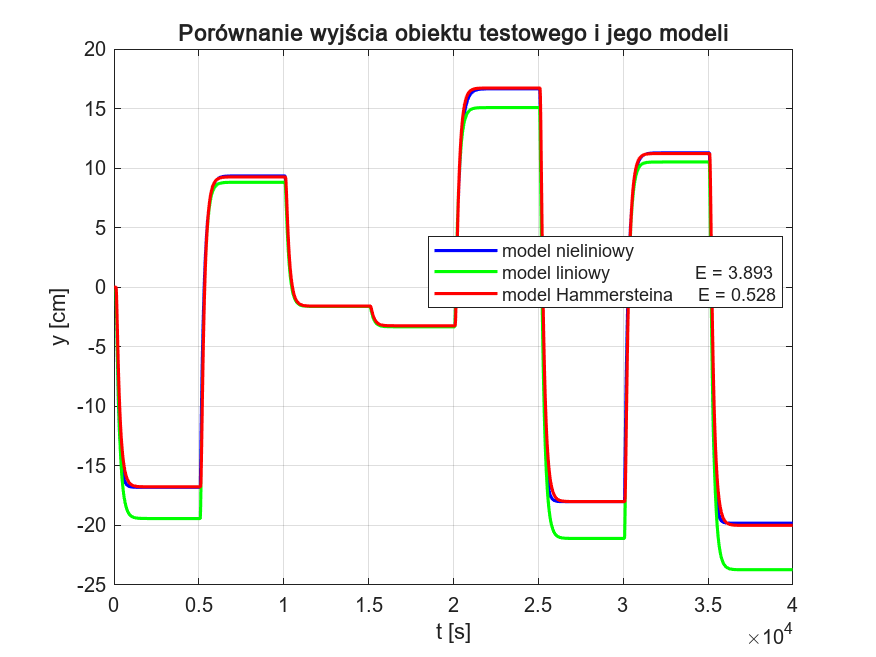
\includegraphics[width=0.75\textwidth]{pictures/HammersteinNonlinearModel_4}}
\caption{Porównanie modelu Hammersteina z następnikami liniowymi i nieliniowymi - czwarta sekwencja.}
\end{figure}

\begin{figure}[p]
\centering
\subfloat[Następniki liniowe]{
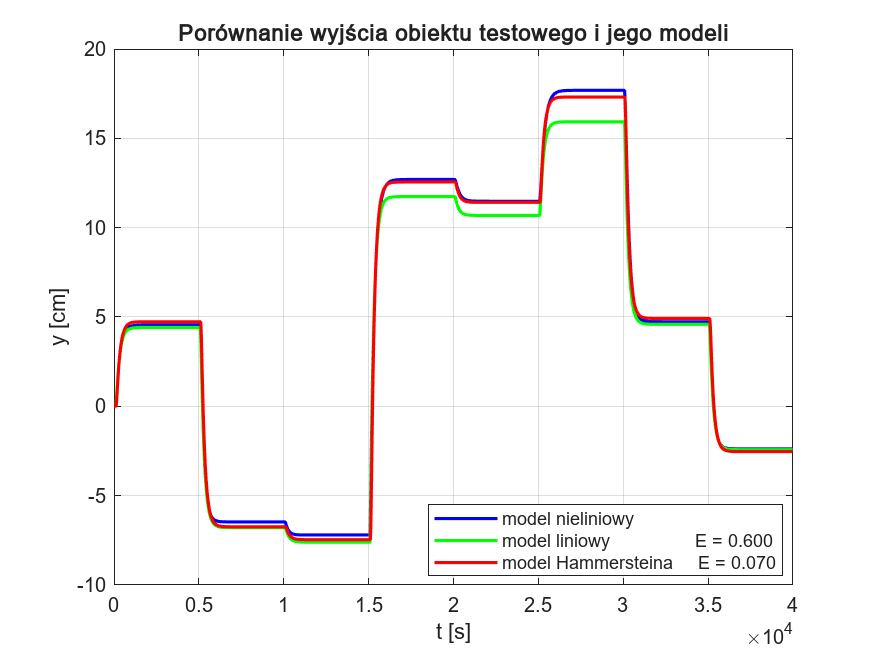
\includegraphics[width=0.75\textwidth]{pictures/HammersteinLinearModel_5}}
\vspace{0.5cm}
\subfloat[Następniki nieliniowe]{
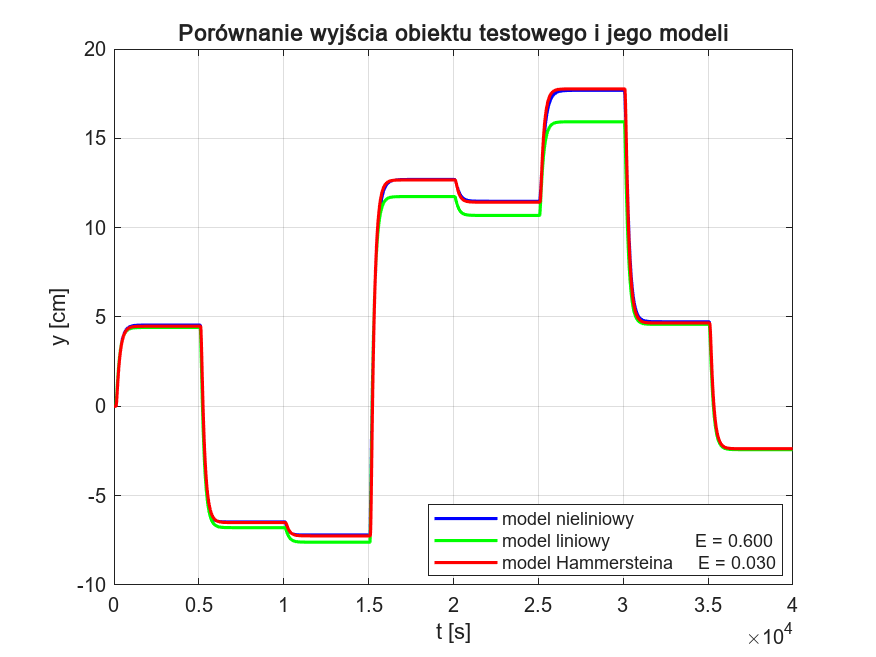
\includegraphics[width=0.75\textwidth]{pictures/HammersteinNonlinearModel_5}}
\caption{Porównanie modelu Hammersteina z następnikami liniowymi i nieliniowymi - piąta sekwencja.}
\label{last_hamm}
\end{figure}

\newpage

Zaprezentowane wykresy na rys. \ref{first_hamm} - \ref{last_hamm} ilustrują przede wszystkim zysk zastosowania modelu Hammersteina do opisu obiektu. Otrzymane wyniki są nieporównywalnie lepsze w stosunku do modelu liniowego. Natomiast przyglądając się z bliska, można zauważyć również poprawę dzięki wprowadzeniu dodatkowej nieliniowości w definicji następników rozmytego modelu typu Takagi-Sugeno. W tab. \ref{comparison_hamm} zebrano uzyskane wyniki.

\begin{table}[h!]
\centering
\renewcommand{\arraystretch}{1.2}
\begin{tabular}{|>{\centering\arraybackslash}m{2cm}|>{\centering\arraybackslash}m{3cm}|>{\centering\arraybackslash}m{3cm}|>{\centering\arraybackslash}m{3cm}|}
\hline
\multirow{2}{*}{Nr sekwencji} & \multirow{2}{*}{Model liniowy} & \multicolumn{2}{c|}{Model Hammersteina} \\ \cline{3-4}
 &  & Następniki liniowe & Następniki nieliniowe \\ \hline
1. & $\num{4.062}$ & $\num{0.395}$ & $\num{0.348}$ \\ \hline
2. & $\num{2.701}$ & $\num{0.210}$ & $\num{0.177}$ \\ \hline
3. & $\num{1.283}$ & $\num{0.146}$ & $\num{0.129}$ \\ \hline
4. & $\num{3.893}$ & $\num{0.597}$ & $\num{0.528}$ \\ \hline
5. & $\num{0.600}$ & $\num{0.070}$ & $\num{0.030}$ \\ \hline
\end{tabular}
\caption{Porównanie modeli.}
\label{comparison_hamm}
\end{table}

Należy pamiętać, że w przypadku następników hiperbolicznych zredukowano liczbę zbiorów rozmytych. Zatem udało się poprawić dokładność modelowania, przy jednoczesnym zmniejszeniu liczby reguł modelu TS.